\chapter{XRM: A Conceptual Model for XR}
\label{ch:conceptual-model}

According to the bibliographical research in \autoref{sec:background-conceptual}, most of the models described are referred to the design of VEs, indeed there are few works dedicated to the design of mixed experiences. This means that existing models are created to meet the needs of a specific application, as the authors continue to build new models from scratch, which are closely tailored to their own domain and therefore difficult to adapt to other applications. The conceptual model should guide designers in the creation and design of multi-reality and multi-platform experiences in order to build a communication bridge between them and the team that has to implement the application. Often these are complex systems combining 3D elements, physical objects, "behaviour-rich content" \cite{walczak_structured_2008}, devices of different nature, single or shared experiences, indoor or outdoor experiences etc. this complexity severely challenge the developers, especially if they are always compelled to intervene directly on the code. 

The XRM Conceptual Model stems from the need to provide a tool capable of covering most of all the technologies included in the Virtual Continuum. The approach used is centered on the human, who is the protagonist in many scenarios thanks to the support of devices and platforms dependent on the environment experienced. The aim is to create a means to enable high-level development of XR applications, in order to involve also non-experts in the domain. 
In the light of the previous comparative and illustrative analysis, from the variety of conceptual models and based on the planned features, the ISS Model was chosen as a starting point for the upcoming model. The model of Gianotti et al.~\cite{dobbie_modeling_2020} provided a dual structure that allows for the systematic design of the static and dynamic parts of an XR experience. Although the context considered have few points in common, the translation of the concepts was not too cumbersome and forced. The XRM Conceptual Model is divided into three parts: a Structural, a Behavioural and an Interaction sub-model, which are described in the next section. 
The Model has been added to the dual structure proposed by the conceptual models analysed in the Comparative study (\autoref{sec:background-conceptual}) with the intention of detailing the concepts separately before combining them. Initially, the elements will be presented by explaining what they represent, their external characteristics and initial properties. Then, user behaviours and effects on technological components will be defined. After that, all the previously defined concepts will be used to compose more or less complex activities that constitute the flow of the experience.


\section{Structural Model}
\label{sec:conceptual-structural}

The Structural Model is the first part of the XRM Conceptual Model. It comprises all participants in the experience, whether implicit or explicit. They constitute the static modeling part, where the components are selected according to the requirements of the application. The structure elected to represent them is a hierarchy of elements with a top-down concreteness approach, whose levels of abstraction are qualitatively marked and identified by a legend of different colors as seen in Figure \autoref{fig:Legend}. The building blocks in the hierarchy are linked by an "is a" relation, which indicates that between two units one of the two is a generalization of the other. In this way the latter is like a  subclass, a child node that inherits from the father \cite{brachman_what_1983}. This implies that the properties owned by a child node will include its own properties in addition to those owned by the father node which are inherited by the child node. Moreover, there is a 'mereology' relation, or so-called composition relation, which is graphically represented with the shape of a full diamond that indicates how a block combined with others can contribute to compose new ones. 

\begin{figure}[h]
	\centering
	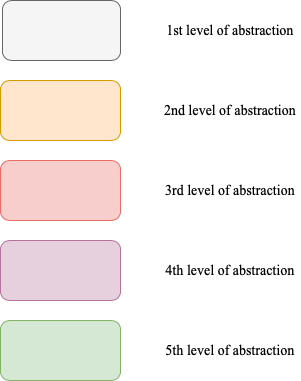
\includegraphics[width=0.5\linewidth]{Figures/Conceptual Model/Legend.png}
	\caption{Legend of levels of abstraction}
	\label{fig:Legend}
\end{figure}

At the summit of the structure stands the entity \emph{Actor}. It embodies a fundamental concept in the field of human-computer interaction, where it is usually considered as a human. In literature it has been defined "as a placeholder for an object when specifying behavior" \cite{de_troyer_conceptual_2007}, i.e. it becomes a way to qualify an abstract object as a system capable of performing actions, stimulating, interacting or reacting to user behavior. The structural model of the XRM Conceptual Model distinguishes in the second abstraction level two macro-categories of Actors as shown in \autoref{fig:ActorHumanNonHuman}.

\begin{figure}[h]
	\centering
	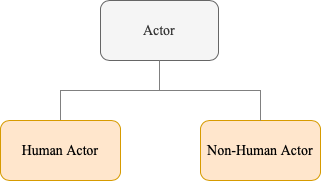
\includegraphics[width=7.5cm]{Figures/Conceptual Model/Actor_Human_NonHuman.png}
	\caption{Structural Model: first two levels of the hierarchy}
	\label{fig:ActorHumanNonHuman}
\end{figure}

\subsection*{Human Actor}
The Human Actor is a type of actor that is generally considered only as a component of the system whose characteristics are crucial in the design process of the interaction with the machine \cite{bannon_discovering_1989}. The presence of a distinction of the Actor between Human and Non-Human arises from the need to elevate the Human from a passive element to an element able to act in an environment, embody and manage a behaviour, rather than being a mere producer of an output information flow. In an interactive system, the Human Actor is nonetheless than the user, the one who uses an application, a device or any technological system through which they perform actions. 

\subsection*{Non-Human Actor}
The Non-Human Actor collects different types of actors, each one with characteristics that must be specified at the design stage. With this term we want to include all the technological components of a system that participate in the interaction allowing the Human Actor to perform certain actions. The results of the interaction are also visible on them.  We can recognize three main sub-categories of Non-Human Actors (\autoref{fig:NonHumanActors}) together with their properties: Physical Component, Environment and Virtual Object.

\begin{figure}[H]
	\centering
	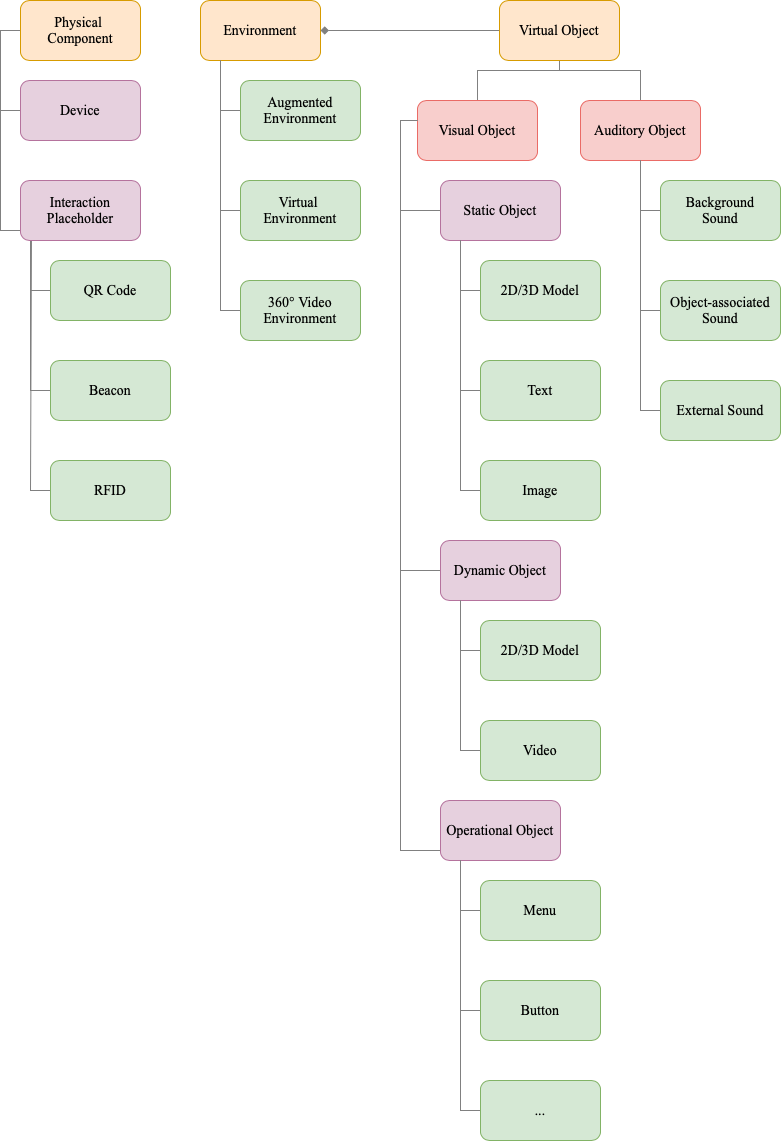
\includegraphics[width=14cm]{Figures/Conceptual Model/NonHumanActors.png}
	\caption{Structural Model - Non-Human Actors hierarchy}
	\label{fig:NonHumanActors}
\end{figure}

\begin{itemize}
    \item \textbf{Physical Component}. Physical Components represent interactive elements with an entirely physical nature, therefore belonging to the real world. They can generate system events or participate in user interactions, receive user commands, trigger other events, etc. \\
    \begin{table}[H]
    \centering
    \begin{tabular}{|l|l|}
    \hline
    \multicolumn{2}{|l|}{\textbf{Physical Component Properties}}                                                                                                \\ \hline
    Id       & It is a unique identification code.                                                                                                              \\ \hline
    Position & \begin{tabular}[c]{@{}l@{}}It is identified by spatial coordinates $(x, y, z)$\\ that locate and track the position of the component.\end{tabular} \\ \hline
    \end{tabular}
    \caption{Structural Model - Physical Component Properties}
    \label{tab:PHCproperties}
    \end{table}
        
    There are two types of Physical Components that we have found:
    \begin{itemize}
        \item \textbf{Interaction Placeholder}. Interaction Placeholders include all identifiable elements i.e. images, codes, symbols such as the QR Code that are recognized by the camera of the device in order to trigger an effect on another Non-Human Actor. However, other devices such as Beacons and RFIDs are also included in this category.
        \item \textbf{Device}: Devices are represented by all the Physical Components that can run an application in XR, whether it is VR or AR. They can be of different nature depending on the technology involved in the designed experience. One or more devices can be included depending on the interaction to be performed. Examples include smartphones, tablets, viewers, card-boards, HMDs, etc.
    \end{itemize}
    \item \textbf{Environment}: Environment represents an element that can have a dual nature. It can identify the real world that can be made of physical objects combined with virtual ones. Otherwise, it can be represented by a world seen through a networked application, a tool supported by a device chosen according to the type of experience designed for the user. In the latter case, the Environment is characterized by a fundamental element: the camera, a device that captures and shows the world to the player. Often the Environment, independently from its nature, is identified with the term "scene", in other cases, instead, the word scene is used to identify the different sub-parts in which it is divided. In this model we will always use only the term 'Environment' in order to avoid any ambiguity. \\
    \begin{table}[H]
    \centering
    \begin{tabular}{|l|l|}
    \hline
    \multicolumn{2}{|l|}{\textbf{Environment Properties}} \\ \hline
    \begin{tabular}[c]{@{}l@{}}Camera \\ Position\end{tabular} &
      \begin{tabular}[c]{@{}l@{}}It is identified by spatial coordinates ($x, y, z$) \\ that locate and track the position of the camera.\end{tabular} \\ \hline
    \begin{tabular}[c]{@{}l@{}}Camera \\ Orientation\end{tabular} &
      \begin{tabular}[c]{@{}l@{}}It is identified by polar coordinates ($\rho$, $\phi$, $\gamma$) \\ that locate and track the camera orientation.\end{tabular} \\ \hline
    Visibility &
      \begin{tabular}[c]{@{}l@{}}It enables or disables the possibility for the user \\ to see the Environment. When in Off mode, the \\ Environment has been triggered but is not visible, \\ i.e. it is hidden from the user's view.\end{tabular} \\ \hline
    \end{tabular}
    \caption{Structural Model - Environment properties}
    \label{tab:Envproperties}
    \end{table}

    The Environment element has three sub-categories:
    \begin{itemize}
        \item \textbf{Augmented Environment}. Augmented Environment (AE) places virtual components in a physical environment. Anchors are virtual elements that the software associates with real elements and that it can recognise, and thus build the experience around the real world by integrating it with the virtual one. Furthermore, AE encapsulates the concept of physical (external) space dimensions, represented as coordinates. It also adds three dimensions where otherwise there would only be one layer superimposed on the users' camera.\\
        \begin{table}[H]
        \centering
        \begin{tabular}{|l|l|}
        \hline
        \multicolumn{2}{|l|}{\textbf{Augmented Environment Properties}}                                                     \\ \hline
        World Anchors & \begin{tabular}[c]{@{}l@{}}They are used by the AR experience\\ to locate the content.\end{tabular} \\ \hline
        \end{tabular}
        \caption{Augmented Environment Properties}
        \label{tab:AEproperties}
        \end{table}
        
        \item \textbf{Virtual Environment}. Virtual Environment  is a completely digital environment that has the characteristic to be navigated and interacted with by the users, of which one or more of their five senses are simulated in real-time \cite{guttentag_virtual_2020}. It places the virtual objects  according to a pure virtual concept of dimensions.
        \begin{table}[H]
        \centering
        \begin{tabular}{|l|l|}
        \hline
        \multicolumn{2}{|l|}{\textbf{Virtual Environment Properties}}                                                       \\ \hline
        World Anchors & \begin{tabular}[c]{@{}l@{}}They are used by the VR experience\\ to locate the content.\end{tabular} \\ \hline
        \end{tabular}
        \caption{Virtual Environment Properties}
        \label{tab:VEproperties}
        \end{table}
        \item \textbf{360$^{\circ}$ Video Environment}. 360$^{\circ}$ Video Environment is represented by a VE that can only be navigated by rotating the device and interacted by buttons superimposed onto the video. The position of the user cannot be changed and overlaps with the position of the camera.\\
        \begin{table}[h]
        \centering
        \begin{tabular}{|l|l|}
        \hline
        \multicolumn{2}{|l|}{\textbf{360$^{\circ}$ Video Environment Properties}}                                           \\ \hline
        Duration & \begin{tabular}[c]{@{}l@{}}It indicates the amount of time\\ the 360$^{\circ}$ Video takes.\end{tabular} \\ \hline
        \end{tabular}
        \caption{360$^{\circ}$ Video Environment Properties}
        \label{tab:360VEproperties}
        \end{table}
    \end{itemize}
    \item \textbf{Virtual Object}. Virtual Object compose the Environment and represent computer-generated elements that simulate real elements and with which the user can interact. Virtual Object in the hierarchy shown (\autoref{fig:NonHumanActors}) is linked to Environment by a "part of" relationship which, as mentioned above, is meant to emphasize that an entity is composed of sub-entities.\\
    \begin{table}[ht]
    \centering
    \begin{tabular}{|l|l|}
    \hline
    \multicolumn{2}{|l|}{\textbf{Virtual Object Properties}}  \\ \hline
    \multirow{4}{*}{Position} &
      \begin{tabular}[c]{@{}l@{}}It is identified by spatial coordinates that \\ locate and track the position of the Virtual Object. \\ These coordinates can be of three types:\end{tabular} \\ \cline{2-2} 
     & Absolute ($x$, $y$, $z$)                               \\ \cline{2-2} 
     & Component-related ($\Delta x$, $\Delta y$, $\Delta z$) \\ \cline{2-2} 
     & User-related ($\Delta x$, $\Delta y$, $\Delta z$)      \\ \hline
    Orientation &
      \begin{tabular}[c]{@{}l@{}}It is identified by polar coordinates ($\rho$, $\phi$, $\gamma$) that \\ locate and track the orientation of the Virtual Object.\end{tabular} \\ \hline
    \end{tabular}
    \caption{Virtual Object Properties}
    \label{tab:VOproperties}
    \end{table}
    Virtual Objects have an additional level of abstraction that characterizes them qualitatively, that is, according to their visual or auditory qualities:
   
   \textbf{Visual Object}. Visual Object encloses a set of Virtual Objects that react to interaction with the user by mainly changing their external characteristics.
    \begin{longtable}[c]{|l|l|l|}
    \hline
    \multicolumn{3}{|l|}{\textbf{Visual Object Properties}} \\ \hline
    \endhead
    %
    \multicolumn{2}{|l|}{Geometry} &
      \begin{tabular}[c]{@{}l@{}}It refers to the representation of the surface, \\ based on mathematical coordinates, that an object \\ can assume. Depending on whether it takes on two or three \\ dimensions, it is called 2D or 3D geometry respectively.\end{tabular} \\ \hline
    \multicolumn{2}{|l|}{Visibility} &
      \begin{tabular}[c]{@{}l@{}}It enables or disables the possibility for the user to see a \\ Visual Object. When in Off mode, the Visual Object has \\ been triggered but is not visible, i.e. it is hidden from \\ the user's view.\end{tabular} \\ \hline
    \multicolumn{2}{|l|}{Scale Factor} &
      \begin{tabular}[c]{@{}l@{}}spatial coordinates (x, y, z) that allow to reduce or increase \\ the size of a Visual Object.\end{tabular} \\ \hline
    \multicolumn{2}{|l|}{Opacity} &
      \begin{tabular}[c]{@{}l@{}}It increases or decreases in percentage the possibility for \\ the user to see a Visual Object. When set to 100\%, the \\ Visual Object has been triggered but is not visible, \\ i.e. it is hidden from the user's view.\end{tabular} \\ \hline
    \multicolumn{2}{|l|}{Selectable} &
      \begin{tabular}[c]{@{}l@{}}It enables or disables the possibility for the user to interact \\ with a Visual Object if the design requires that the object be \\ selected before an action can be performed. When in Off mode, \\ the Visual Object is visible but not interactive, \\ i.e. it does not respond to user commands.\end{tabular} \\ \hline
    \multicolumn{2}{|l|}{Blinking} &
      \begin{tabular}[c]{@{}l@{}}It enables or disables the possibility for the user to see a \\ Visual Object surrounded by a luminous border. When in \\ Off mode, the Visual Object is visible but the luminous border \\ is hidden from the user. This is used, for example, to draw the \\ user's attention to a certain object.\end{tabular} \\ \hline
     &
      Frequency &
      \begin{tabular}[c]{@{}l@{}}It determines the number of times the Visual Object blinks \\ per unit of time.\end{tabular} \\ \hline
     &
      Colour &
      \begin{tabular}[c]{@{}l@{}}It represents the chromatic shade that the light around the \\ Visual Object takes on.\end{tabular} \\ \hline
    \caption{Visual Object Properties}
    \label{tab:VIOtable}\\
    \end{longtable}
    Visual Objects are divided into three subsets: 
    \begin{itemize}
        \item \textbf{Static Object}. Static Object is a Visual Object that is not characterised by movement or animation. We distinguish three types of Static Objects:
        \begin{itemize}
            \item \textbf{2D/3D Model}: 2D/3D Model is a mathematical representation of a two- or three-dimensional object, i.e. a 2D/3D computer-generated geometry.
            \begin{table}[h]
            \centering
            \begin{tabular}{|l|l|}
            \hline
            \multicolumn{2}{|l|}{\textbf{2D/3D Model Properties}} \\ \hline
            Texture &
              \begin{tabular}[c]{@{}l@{}}It is a two-dimensional image in raster format that is \\ reproduced on one or more faces of a multidimensional model. \\ It corresponds to the chromatic variations \\ that a Model may present on the surface.\end{tabular} \\ \hline
            \end{tabular}
            \caption{2D/3D Model Properties}
            \label{tab:2d3dMproperties}
            \end{table}
            \item \textbf{Image}: Image is a visual representation enclosed in a two-dimensional window
            \item \textbf{Text}: Text is a visual description enclosed in a two-dimensional window.\\
            \begin{table}[H]
            \centering
            \begin{tabular}{|l|l|}
            \hline
            \multicolumn{2}{|l|}{\textbf{Text Properties}} \\ \hline
            Offset &
              \begin{tabular}[c]{@{}l@{}}it increases or decreases the user's ability \\ to see Text. When Offset is not set to 100\%, \\ the Text has been triggered but is not visible in full, \\ i.e. a portion is hidden from the user's view.\end{tabular} \\ \hline
            Language &
              \begin{tabular}[c]{@{}l@{}}It allows the user to switch the translation of the \\ Text based on user preferences.\end{tabular} \\ \hline
            \end{tabular}
            \caption{Text Properties}
            \label{tab:Textproperties}
            \end{table}
        \end{itemize}
        \item \textbf{Dynamic Object}. Dynamic Object is a Visual Object that is characterised by movement or animation.\\
        \begin{table}[H]
        \centering
        \begin{tabular}{|l|l|}
        \hline
        \multicolumn{2}{|l|}{\textbf{Dynamic Properties}}                                                                        \\ \hline
        Loop     & \begin{tabular}[c]{@{}l@{}}It enables the cyclic reproduction of a \\ Dynamic Object.\end{tabular} \\ \hline
        Duration & \begin{tabular}[c]{@{}l@{}}It keeps updates the amount of play time of a \\ Dynamic Object.\end{tabular}        \\ \hline
        \end{tabular}
        \caption{Dynamic Properties}
        \label{tab:Dynproperties}
        \end{table}
        There are two types of Dynamic Objects:
        \begin{itemize}
            \item \textbf{2D/3D Model}. 2D/3D Model is a mathematical representation of a two-dimensional/three-dimensional object, i.e. a 2D/3D computer-generated geometry.
            \item \textbf{Video}. Video is a visual reproduction represented in a two-dimensional window.
        \end{itemize}
        \item \textbf{Operational Object}. Operational Object is a Visual Object that allows operations to be carried out and commands to be sent to the system by the user. There are two examples of Operational Objects:
        \begin{itemize}
            \item \textbf{Menu}. Menu consists of a list of elements that can trigger a change of state through a graphical interface, whose geometry can be either 2D or 3D.
            \item \textbf{Button}: Button is a component of the Menu, it allows the user to trigger an event.
        \end{itemize}
    \end{itemize}
    
    \textbf{Auditory Object}. Auditory Object encloses a set of objects that react to interaction with the user with a change in their sound characteristics.\\
	\begin{table}[H]
    \centering
    \begin{tabular}{|l|l|}
    \hline
    \multicolumn{2}{|l|}{\textbf{Auditive Properties}}                                                                                      \\ \hline
    Mute &
      \begin{tabular}[c]{@{}l@{}}It enables or disables the possibility for the user \\ to listen to an Auditory Object. When in Off mode, \\ the Auditory Object has been triggered but cannot \\ be listened to.\end{tabular} \\ \hline
    Duration & \begin{tabular}[c]{@{}l@{}}It allows the user to switch the language of the \\ sound based on user preferences.\end{tabular} \\ \hline
    Loop     & It enables the cyclic playback of an Auditory Object.                                                                        \\ \hline
    \end{tabular}
    \caption{Auditive Properties}
    \label{tab:Audproperties}
    \end{table}
    Auditory Objects are distinguished on the basis of the source from which the sound is reproduced:
    \begin{itemize}
        \item \textbf{Background Sound}: Background Sound is a secondary sound that is activated to complement the experience or part of it, it can be for example a soundtrack etc.
        \item \textbf{Object-associated Sound}: Object-associated Sound is a sound that is linked to the object with which the user is interacting, it can be for example a short sound that provides feedback to indicate the status of the action carried out, such as a timer that signals that time is up.
        \item \textbf{External Sound}: External Sound is a sound from a third party source such as the voice of the tour guide etc.
    \end{itemize}
\end{itemize}

\section{Behavioral Model}
\label{sec:conceptual-behavioral}
\section{Interaction Model}
\label{sec:conceptual-interaction}

The Interaction Model is the third part of the XRM conceptual model. The Behavioural Model focused on defining the capabilities of Actors according to their roles.  Based on it, the Interaction Model aims to combine the different actions of users, the Target of these actions, and how one or more Actuators respond to this interaction.
Similar to the Behavioural Model, the Interaction Model defines primitives: the Interaction and the System Event.
In addition, it includes two sub-models distinguished by the level of abstraction. The one at a lower level aims to compose a more complex system starting from the primitives just defined: the Task. At a high level, on the other hand, the Activity is composed of a concatenation of Tasks and aims to provide a complete picture of the flow of the experience. 

\subsection*{Design of the Task: Low-Level Conceptualization}

In order to give a more exhaustive definition of the concept of Task, it is first required to explore two fundamental elements: Interaction and the System Event.

\subsubsection*{Interaction}

The \emph{Interaction} represents a process where a Human Actor performs actions on a Non-Human Actor, the Actuator, to complete a task. Each interaction is defined by the User’s Actions. 
An Interaction is to be considered within the Interaction Model as a building block that contains the three primitives analysed in the Behavioural Model (\autoref{sec:conceptual-behavioral}).  
It must be a non-null set. The Non-Human Actors involved may be one or more than one in the case of a more complex Interaction and the Human Actor, which is the one that initiates the Interaction, cannot be omitted from the design. It is hard to provide a list of interactions because the combinations would be too many, so we distinguish some built-in interactions and their behaviour related to the Device involved:
\begin{table}[h]
\centering
\begin{tabular}{|l|l|}
\hline
\multicolumn{2}{|l|}{\textbf{Interaction}} \\ \hline
Take Screenshot & \begin{tabular}[c]{@{}l@{}}It represents an instant capture of the displayed \\ Environment or Virtual Object.\end{tabular} \\ \hline
Record View     & \begin{tabular}[c]{@{}l@{}}It represents a recording of the displayed \\ Environment or Virtual Object.\end{tabular}        \\ \hline
Save Acquisition & \begin{tabular}[c]{@{}l@{}}It represents that a screenshot or recording is \\ saved on the Device in use.\end{tabular}      \\ \hline
Dictation       & \begin{tabular}[c]{@{}l@{}}It represents that the user’s voice is recognized \\ by the Device.\end{tabular}                 \\ \hline
\end{tabular}
\caption{Interaction - graphical representation}
\label{tab:InteractionTable}
\end{table}
As can be seen from Figure \autoref{fig:InteractionBlock}, it shows the three main components contained within our building block, which can be renamed by the designer with a title that briefly explains the intended interaction.

\begin{figure}[h]
	\centering
	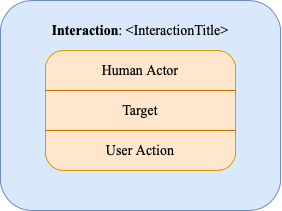
\includegraphics[width=7.5cm]{Figures/Conceptual Model/InteractionBlock.png}
	\caption{Interaction - graphical representation}
	\label{fig:InteractionBlock}
\end{figure}

Some examples of interactions that can be created and customised according to the experience are given below: 
\begin{itemize}
    \item The experience designer can model a "Proximity In" interaction involving the user as a Human Actor, the Walk In action as a User Action and the Virtual Object as an Actuator. 
    \item The experience designed using HMDs allows the user to interact with the Virtual Object by tapping (User Action: Tap) on a 3D Model (Actuator) to "Select the Object" (Effect). A subsequent Tap allows the user the next interaction, for example to play the content. 
\end{itemize}

\subsubsection*{System Event}

The \emph{System Event} provides the signal that triggers the event call. The stimuli generated by the events are, of course, outside the direct control of the user \autoref{fig:SystemEvent}.
\begin{figure}[h]
	\centering
	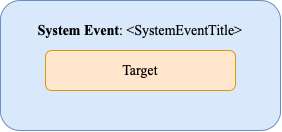
\includegraphics[width=7.5cm]{Figures/Conceptual Model/SystemEvent.png}
	\caption{System Event - graphical representation}
	\label{fig:SystemEvent}
\end{figure}
The System Event is a building block in the same way as the Interaction block, with the difference that neither the Human Actor nor the User Action appears. The only element contained in the System Event block is the Non-Human Actor that participates in the System generated Event.
An example of a System Event is the Beacon Reception. This is a Bluetooth-based technology that allows Bluetooth devices to transmit and receive small messages within short distances. The system is able to recognise the wireless device and the effects triggered can be multiple and show up on one or more Non-Human Actors. 

\subsubsection*{Task}

\emph{Task} is defined as an interaction or system event that generates an effect. \autoref{fig:Task} shows how it embeds two blocks connected by an arrow, recalling a cause-and-effect scenario.
\begin{figure}[h]
	\centering
	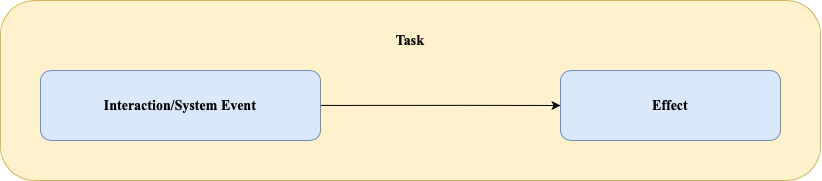
\includegraphics[width=12cm]{Figures/Conceptual Model/Task.png}
	\caption{Task - graphical representation}
	\label{fig:Task}
\end{figure}
The Task can be either user or system dependent. It is described by a sub-model using the building blocks presented so far. 
The user-dependent Task is represented by the presence of the Interaction block, which defines the User Actions that the user can do on one or more Non-Human Actors, combined with the Effects generated on one or more Non-Human Actors. Interactions are seen in detail with respect to the higher level sub-model which will be described later. 
A Task that depends on a System Event defines perceptible Effects on the system and the environment. A change in state of a system device (e.g., "increase in display brightness") is not generated as a response to explicit and intentional human actions in the XR experience, but instead results from phenomena perceived by Non-Human Actors, such as common devices like our smartphones that recognise the decrease in natural light.
At this level, the general purpose of the Task is set out with a representative sentence devised by the experience designer. The composition of the Task should be quite intuitive and straightforward after defining its atomic components individually.
By combining primitives representing an interaction (Human Actor, User Action, Target) or a System Event (Target) it is possible to associate the Effect that is generated on the Actuator. The following table shows an example overview of the many possible combinations. 
%% PHYSICAL COMPONENT

\begin{table}[h]
\centering
\begin{tabular}{|c|c|c|c|c|c|}
\hline
\rowcolor[HTML]{DAE8FC} 
\multicolumn{4}{|l|}{\cellcolor[HTML]{DAE8FC}{\color[HTML]{333333} Interaction/System Event}} &
  \multicolumn{2}{l|}{\cellcolor[HTML]{DAE8FC}{\color[HTML]{333333} Effect}} \\ \hline
\rowcolor[HTML]{FFE6CC} 
\multicolumn{1}{|l|}{\cellcolor[HTML]{FFE6CC}\begin{tabular}[c]{@{}l@{}}Human\\ Actor\end{tabular}} &
  \multicolumn{1}{l|}{\cellcolor[HTML]{FFE6CC}\begin{tabular}[c]{@{}l@{}}User\\ Action\end{tabular}} &
  \multicolumn{2}{l|}{\cellcolor[HTML]{FFE6CC}Target} &
  \multicolumn{1}{l|}{\cellcolor[HTML]{DAE8FC}} &
  \multicolumn{1}{l|}{\cellcolor[HTML]{DAE8FC}Actuator} \\ \hline
 &
  \begin{tabular}[c]{@{}c@{}}Press, \\ Click, \\ Speak\end{tabular} &
  Device &
   &
  \begin{tabular}[c]{@{}c@{}}Screenshot Acquisition,\\ Recording Acquisition,\\ Acquired Element saved,\\ Speech to text\end{tabular} &
  Device \\ \cline{2-6} 
 &
  Frame &
   &
  QR Code &
   &
  \begin{tabular}[c]{@{}c@{}}Device, \\ E, VO\end{tabular} \\ \cline{2-2} \cline{4-4} \cline{6-6} 
\multirow{-3}{*}{User U} &
  Frame &
   &
  RFID &
   &
  \begin{tabular}[c]{@{}c@{}}Device,\\ E, VO\end{tabular} \\ \cline{1-2} \cline{4-4} \cline{6-6} 
- &
  - &
  \multirow{-3}{*}{\begin{tabular}[c]{@{}c@{}}Interaction\\ Placholder \\ (IP)\end{tabular}} &
  Beacon &
  \multirow{-3}{*}{Show, Hide} &
  \begin{tabular}[c]{@{}c@{}}Device,\\ E, VO\end{tabular} \\ \hline
\end{tabular}
\caption{ Task Combination - Physical Components (PHC)}
\label{tab:PHCtask}
\end{table}

%% ENVIRONMENT

\begin{table}[h]
\centering
\begin{tabular}{|c|c|c|c|c|}
\hline
\rowcolor[HTML]{DAE8FC} 
\multicolumn{3}{|l|}{\cellcolor[HTML]{DAE8FC}{\color[HTML]{333333} Interaction/System Event}} &
  \multicolumn{2}{l|}{\cellcolor[HTML]{DAE8FC}{\color[HTML]{333333} Effect}} \\ \hline
\rowcolor[HTML]{FFE6CC} 
\multicolumn{1}{|l|}{\cellcolor[HTML]{FFE6CC}\begin{tabular}[c]{@{}l@{}}Human\\ Actor\end{tabular}} &
  \multicolumn{1}{l|}{\cellcolor[HTML]{FFE6CC}\begin{tabular}[c]{@{}l@{}}User\\ Action\end{tabular}} &
  \multicolumn{1}{l|}{\cellcolor[HTML]{FFE6CC}Target} &
  \multicolumn{1}{l|}{\cellcolor[HTML]{DAE8FC}} &
  \multicolumn{1}{l|}{\cellcolor[HTML]{DAE8FC}Actuator} \\ \hline
 &
  Walk In &
   &
  Show, Hide &
   \\ \cline{2-2} \cline{4-4}
 &
  Walk Out &
  \multirow{-2}{*}{\begin{tabular}[c]{@{}c@{}}Augmented\\ Environment\end{tabular}} &
  Show, Hide &
  \multirow{-2}{*}{E, VO} \\ \cline{2-5} 
 &
  Walk In &
   &
  Show, Hide &
   \\ \cline{2-2} \cline{4-4}
 &
  Walk Out &
  \multirow{-2}{*}{\begin{tabular}[c]{@{}c@{}}Virtual\\ Environment\end{tabular}} &
  Show, Hide &
  \multirow{-2}{*}{E, VO} \\ \cline{2-5} 
\multirow{-5}{*}{User U} &
  \multicolumn{1}{l|}{Look Around} &
  \multicolumn{1}{l|}{\begin{tabular}[c]{@{}l@{}}360° Video \\ Environment\end{tabular}} &
  \multicolumn{1}{l|}{Change User View} &
  \multicolumn{1}{l|}{E, VO} \\ \hline
\end{tabular}
\caption{ Task Combination - Environment (E)}
\label{tab:Envtask}
\end{table}

%% VIRTUAL OBJECT - VISUAL OBJECT
\begin{table}[]
\centering
\begin{tabular}{|c|c|c|c|c|c|c|}
\hline
\rowcolor[HTML]{DAE8FC} 
\multicolumn{5}{|l|}{\cellcolor[HTML]{DAE8FC}{\color[HTML]{333333} Interaction/System Event}} &
  \multicolumn{2}{l|}{\cellcolor[HTML]{DAE8FC}{\color[HTML]{333333} Effect}} \\ \hline
\rowcolor[HTML]{FFE6CC} 
\multicolumn{1}{|l|}{\cellcolor[HTML]{FFE6CC}\begin{tabular}[c]{@{}l@{}}Human\\ Actor\end{tabular}} &
  \multicolumn{1}{l|}{\cellcolor[HTML]{FFE6CC}\begin{tabular}[c]{@{}l@{}}User\\ Action\end{tabular}} &
  \multicolumn{3}{l|}{\cellcolor[HTML]{FFE6CC}Target} &
  \multicolumn{1}{l|}{\cellcolor[HTML]{DAE8FC}} &
  \multicolumn{1}{l|}{\cellcolor[HTML]{DAE8FC}Actuator} \\ \hline
 &
  \begin{tabular}[c]{@{}c@{}}Tap, \\ Press, \\ Click\end{tabular} &
   &
   &
   &
  \begin{tabular}[c]{@{}c@{}}Select\\ Component\end{tabular} &
   \\ \cline{2-2} \cline{6-6}
 &
  \begin{tabular}[c]{@{}c@{}}Gaze In \\ and Dwell\end{tabular} &
   &
   &
   &
   &
   \\ \cline{2-2}
 &
  Walk In &
   &
   &
   &
  \multirow{-2}{*}{Show} &
   \\ \cline{2-2} \cline{6-6}
 &
  Gaze Out &
   &
   &
   &
   &
   \\ \cline{2-2}
 &
  Walk Out &
   &
  \multirow{-5}{*}{} &
  \multirow{-5}{*}{} &
  \multirow{-2}{*}{Hide} &
  \multirow{-5}{*}{E, VO} \\ \cline{2-2} \cline{4-7} 
 &
   &
   &
   &
   &
  \begin{tabular}[c]{@{}c@{}}Change \\ Position\end{tabular} &
   \\ \cline{6-6}
 &
   &
   &
   &
   &
  \begin{tabular}[c]{@{}c@{}}Change\\ Scale Factor\end{tabular} &
   \\ \cline{6-6}
 &
   &
   &
   &
   &
  \begin{tabular}[c]{@{}c@{}}Change\\ Orientation\end{tabular} &
   \\ \cline{6-6}
 &
  \multirow{-4}{*}{Manipulate} &
   &
   &
  \multirow{-4}{*}{} &
  \begin{tabular}[c]{@{}c@{}}Change\\ Texture\end{tabular} &
  \multirow{-4}{*}{VO} \\ \cline{2-2} \cline{5-7} 
 &
   &
   &
   &
  Model &
   &
   \\ \cline{2-2} \cline{5-6}
 &
   &
   &
   &
   &
  \begin{tabular}[c]{@{}c@{}}Change \\ Offset\end{tabular} &
   \\ \cline{6-6}
 &
  \multirow{-2}{*}{Swipe} &
   &
   &
  \multirow{-2}{*}{Text} &
  \begin{tabular}[c]{@{}c@{}}Change\\ Language\end{tabular} &
   \\ \cline{2-2} \cline{5-6}
 &
   &
   &
  \multirow{-8}{*}{\begin{tabular}[c]{@{}c@{}}Static \\ Object\\ (SO)\end{tabular}} &
  Image &
  \begin{tabular}[c]{@{}c@{}}Change\\ Image\end{tabular} &
   \\ \cline{2-2} \cline{4-6}
 &
   &
   &
   &
   &
  Play &
   \\ \cline{6-6}
 &
   &
   &
   &
   &
  Pause &
   \\ \cline{6-6}
 &
   &
   &
   &
  \multirow{-3}{*}{} &
  \begin{tabular}[c]{@{}c@{}}Playback\\ Control\end{tabular} &
   \\ \cline{5-6}
 &
   &
   &
   &
  Model &
   &
   \\ \cline{5-6}
 &
  \multirow{-5}{*}{Swipe} &
   &
  \multirow{-5}{*}{\begin{tabular}[c]{@{}c@{}}Dynamic\\ Object \\ (DO)\end{tabular}} &
  Video &
   &
  \multirow{-9}{*}{VO} \\ \cline{2-2} \cline{4-7} 
\multirow{-19}{*}{User U} &
   &
  \multirow{-19}{*}{\begin{tabular}[c]{@{}c@{}}Visual \\ Object\\ (VO)\end{tabular}} &
  \begin{tabular}[c]{@{}c@{}}Operational\\ Object \\ (OO)\end{tabular} &
   &
  \begin{tabular}[c]{@{}c@{}}Active\\ Custom\\ Action\end{tabular} &
  E, VO \\ \hline
\end{tabular}
\caption{ Task Combination - Virtual Object (VO), Visual Object (VIO)}
\label{tab:VIOTask}
\end{table}

%% VIRTUAL OBJECT - AUDITORY OBJECT
\begin{table}[]
\centering
\begin{tabular}{|c|c|c|c|c|c|}
\hline
\rowcolor[HTML]{DAE8FC} 
\multicolumn{4}{|l|}{\cellcolor[HTML]{DAE8FC}{\color[HTML]{333333} Interaction/System Event}} &
  \multicolumn{2}{l|}{\cellcolor[HTML]{DAE8FC}{\color[HTML]{333333} Effect}} \\ \hline
\rowcolor[HTML]{FFE6CC} 
\multicolumn{1}{|l|}{\cellcolor[HTML]{FFE6CC}\begin{tabular}[c]{@{}l@{}}Human\\ Actor\end{tabular}} &
  \multicolumn{1}{l|}{\cellcolor[HTML]{FFE6CC}\begin{tabular}[c]{@{}l@{}}User\\ Action\end{tabular}} &
  \multicolumn{2}{l|}{\cellcolor[HTML]{FFE6CC}Target} &
  \multicolumn{1}{l|}{\cellcolor[HTML]{DAE8FC}} &
  \multicolumn{1}{l|}{\cellcolor[HTML]{DAE8FC}Actuator} \\ \hline
 &
  \begin{tabular}[c]{@{}c@{}}Effects on \\ AO correspond\\ to User Actions\\ on other \\ Actors\end{tabular} &
  \begin{tabular}[c]{@{}c@{}}Auditory \\ Object\\ (AO)\end{tabular} &
   &
  \begin{tabular}[c]{@{}c@{}}Play,\\ Pause,\\ Change\\ Language,\\ Playback\\ Control,\\ Audio\\ Control\end{tabular} &
  Device, VO \\ \cline{2-6} 
 &
   &
   &
  \begin{tabular}[c]{@{}c@{}}Background\\ Sound\end{tabular} &
   &
  Device, VO \\ \cline{2-6} 
 &
   &
   &
  \begin{tabular}[c]{@{}c@{}}Object-associated\\ Sound\end{tabular} &
   &
  VO \\ \cline{2-6} 
\multirow{-4}{*}{User U} &
   &
   &
  \begin{tabular}[c]{@{}c@{}}External\\ Source\end{tabular} &
   &
  Device, VO \\ \hline
\end{tabular}
\caption{ Task Combination - Virtual Object (VO), Auditory Object (AO)}
\label{tab:AOTask}
\end{table}

\subsection*{Design of the Activity: High-Level Conceptualization}

The high-level Activity conceptualisation sub-model is defined as a compression of the low-level conceptualisation sub-model. It attempts to organise the individual Tasks and specifically the interactions and related effects, so as to construct a sequence that leads the user to the achievement of a particular end. This model does not go into detail about the individual elements that compose it, but rather aims to design the series of steps that the user must complete in order to reach the goal. 

\subsubsection*{Activity}

The \emph{Activity} is defined as a flow of Tasks. The description of the flow defines the order in which the Tasks must be executed to build the whole experience. Figure \autoref{fig:Activity} represents the Activity as a collector of Tasks, from the starting Task 0, to the N-th Task that marks the conclusion of the single Activity. 
\begin{figure}[h]
	\centering
	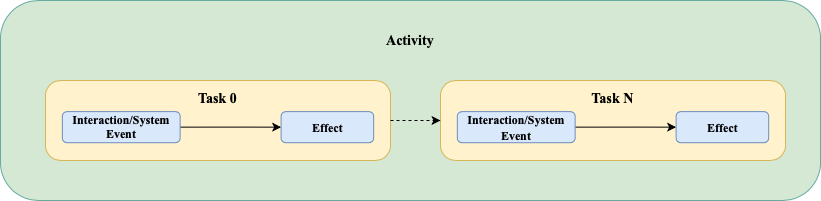
\includegraphics[width=13cm]{Figures/Conceptual Model/Activity.png}
	\caption{Activity: graphical representation}
	\label{fig:Activity}
\end{figure}
To describe the sequence of the actions we decided to use a well-known notation, namely the concepts derived from the BPMN 2.0 model.
The BPMN notation \footnote{http://www.bpmn.org} was developed by the "Business Process Management Initiative" and the "Object Management Group" \footnote{http://www.omg.org}, non-profit associations bringing together operators in the field of information technology and organisational analysis. The BPMN aims to provide an effective representation standard that is easy to use and understand by business users interested in the problem of modelling, design and possible digitalisation of business processes.
The BPMN is essentially a derivation of the formalism of flow charts but with some additions and modifications that make it possible to overcome certain limitations in the modelling of business processes. It makes it possible to construct business process diagrams (BPD) that represent graphs or networks made up of "objects" represented by the process operations, connected by control flows that define the logical relationship, dependencies and order of execution of the operations themselves. 
The BPMN standard defines some basic graphical elements, divided into four categories. We have imported and re-adapted, according to our needs, only two of these categories, considered fundamental to describe the Activities of our model: flow and connecting objects. Flow objects include:
\begin{itemize}
    \item Event: The Event is represented by a circle (\autoref{fig:ActivityElements}) and represents something that happens during a process. Events can have a "cause" that triggers them and a possible "outcome". There are three types of events depending on their location within the flow of a process: start, intermediate and end.
    \item Node: The Node is represented with a blunt rectangle, indicating what we have previously defined as a Task that is carried out within the process considered (\autoref{fig:ActivityElements}). In the official BMPN 2.0 version the Node is called Activity. To avoid ambiguity with the Activity we defined as a flow of Tasks, we chose the term Node. Moreover, a Node represents an elementary and "atomic" entity, i.e. not further decomposable, the BMPN Activity, instead, can also include complex tasks.
    \begin{figure}[H]
	\centering
	
\includegraphics[width=12cm]{Figures/Conceptual Model/ActivityElements.png}
	\caption{Activity Flow Objects - Event, Node and Sequence flow}
	\label{fig:ActivityElements}
    \end{figure}

    \item Gateway: The Gateway is represented by a rhombus (\autoref{fig:Gateways}), it defines the points of the Activity where Task flows diverge or converge. It is used to represent traditional decision points as in classic flow charts, but also simple bifurcations of the Task flow into parallel Tasks or conversely the rejoining of parallel Tasks into a single flow. In other words, Gateways alter the normal direct temporal sequences determined by simple connecting elements, introducing the notion of parallelism, synchronisation and alternative paths. Let us consider the following types of gateway:
    \begin{itemize}
        \item Exclusive: Used to create alternative flows in a Activity. Since only one of the paths can be taken, once a Task has been executed, the others can no longer be executed.
        \item Event-driven: the condition that determines the Task to be executed is based on an evaluated event, a condition on the state of the system to be respected.
        \item Parallel: links several Tasks and indicates that each of them can be executed in parallel without evaluating any condition.
        \item Inclusive: used to create alternative flows in which all tasks are evaluated.
    \end{itemize}
    \begin{figure}[H]
	\centering
	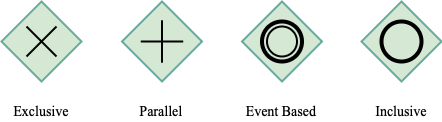
\includegraphics[width=10cm]{Figures/Conceptual Model/Gateways.png}
	\caption{Activity Flow Objects - Gateways}
	\label{fig:Gateways}
    \end{figure}
    
\end{itemize}
In a process the flow elements (events, nodes or gateways) represent "what actually happens" so they must be logically connected to each other. This is what connectors are for. 

\begin{itemize}
    \item Sequence flow: is drawn with a filled arrow \autoref{fig:Activity} and is used to indicate the logical-sequential order between Nodes and Events. 
\end{itemize}

\section{Example of use of XRM: The NURE Use Case}
\label{sec:conceptual-nure-example}